% Chapter 1: Introduction
\chapter{Introduction}\label{chap:introduction}
\section{Background and Motivation}

Automatic readability assessment is now an important research topic in Natural Language Processing (NLP) and in educational technology \cite{dubay2004principles}. Readability assessment tries to determine how difficult a text is for a specific group of readers. These systems are useful in education, for example in intelligent tutoring systems, curriculum design and text simplification~\cite{vajjala2022trends}.

Arabic readability assessment is still a hard task because Arabic is linguistically complex, with rich morphology, flexible syntax and a good deal of lexical ambiguity \cite{nassiri2023approaches}. Deep learning and transformer based language models have advanced a lot in recent years, but fine grained Arabic readability prediction has received much less attention than English and other languages.

The Balanced Arabic Readability Evaluation Corpus (BAREC) recently introduced a large scale benchmark for Arabic readability assessment. It contains 69,441 sentences spread over 19 readability levels, which are named in the Abjad order of the Arabic letters (1-\textit{alif} through 19-\textit{qaf}), and ranging from kindergarten to postgraduate comprehension \cite{elmadani2025barec}. The corpus provides an essential resource for evaluating modern deep learning approaches to Arabic readability modeling. Its release was accompanied by the BAREC 2025 Shared Task \cite{elmadani2025sharedtask}, in which several systems tried ordinal aware modeling, among them the ZAI system, which used AraBERTv2 with a CORAL ordinal head~\cite{nazzal2025zai}, and the STBW system, which used a two-phase MSE/Soft-QWK training strategy \cite{trigui2025stbw}.

Most traditional classification approaches treat readability labels as independent classes and ignore the order between levels. Readability levels are ordered by nature, though. When the true level is 7, predicting level 8 is off by one grade, while predicting level 1 would put a second grade text at kindergarten level. Standard Cross Entropy loss penalizes both errors the same way and so throws away the ordering information in the labels. This is the reason for using ordinal regression methods and distance aware loss functions \cite{castagnos2022ordinal}.

In this work we compare twelve head and loss configurations under one identical pipeline: cross entropy, regression with mean squared error, ordinal log loss, an Earth Mover's Distance loss, four soft label settings, a CORAL ordinal head, two regression losses with a pairwise ranking term (RANK and PLR) and a conditional ordinal head (CORN). These last three come from outside the BAREC benchmark: RANK and PLR from readability research on other languages \cite{trokhymovych2024open,lee2022neural}, and CORN from ordinal regression \cite{shi2023deep}. None of the three was evaluated in the BAREC benchmark or by the ZAI and STBW systems. We also include a Soft QWK schedule in two phases, reported as its own group because its training schedule is different. AraBERTv2 with D3Tok morphological segmentation is the fixed backbone, the BAREC corpus is the benchmark and quadratic weighted kappa is the metric. A second track freezes the encoder and trains only a linear head on cached features. It runs in minutes on a laptop processor, which satisfies the CPU friendly setting the research topic asks for, and we repeat it over five seeds so that we can report variance.
\section{Challenges in Arabic Readability Assessment}
Arabic readability assessment is a hard task for several linguistic and computational reasons. Compared with English, Arabic has a rich morphology, a flexible sentence structure and a high degree of lexical ambiguity, and all of these make automatic text processing more difficult.
The first difficulty is morphology. An Arabic word is often built from a root with prefixes, suffixes and clitics attached, so the same word appears in many forms and lexical representations become sparse. As a result, tokenization and feature extraction are harder than in many other languages.
\begin{figure}[H]

\centering

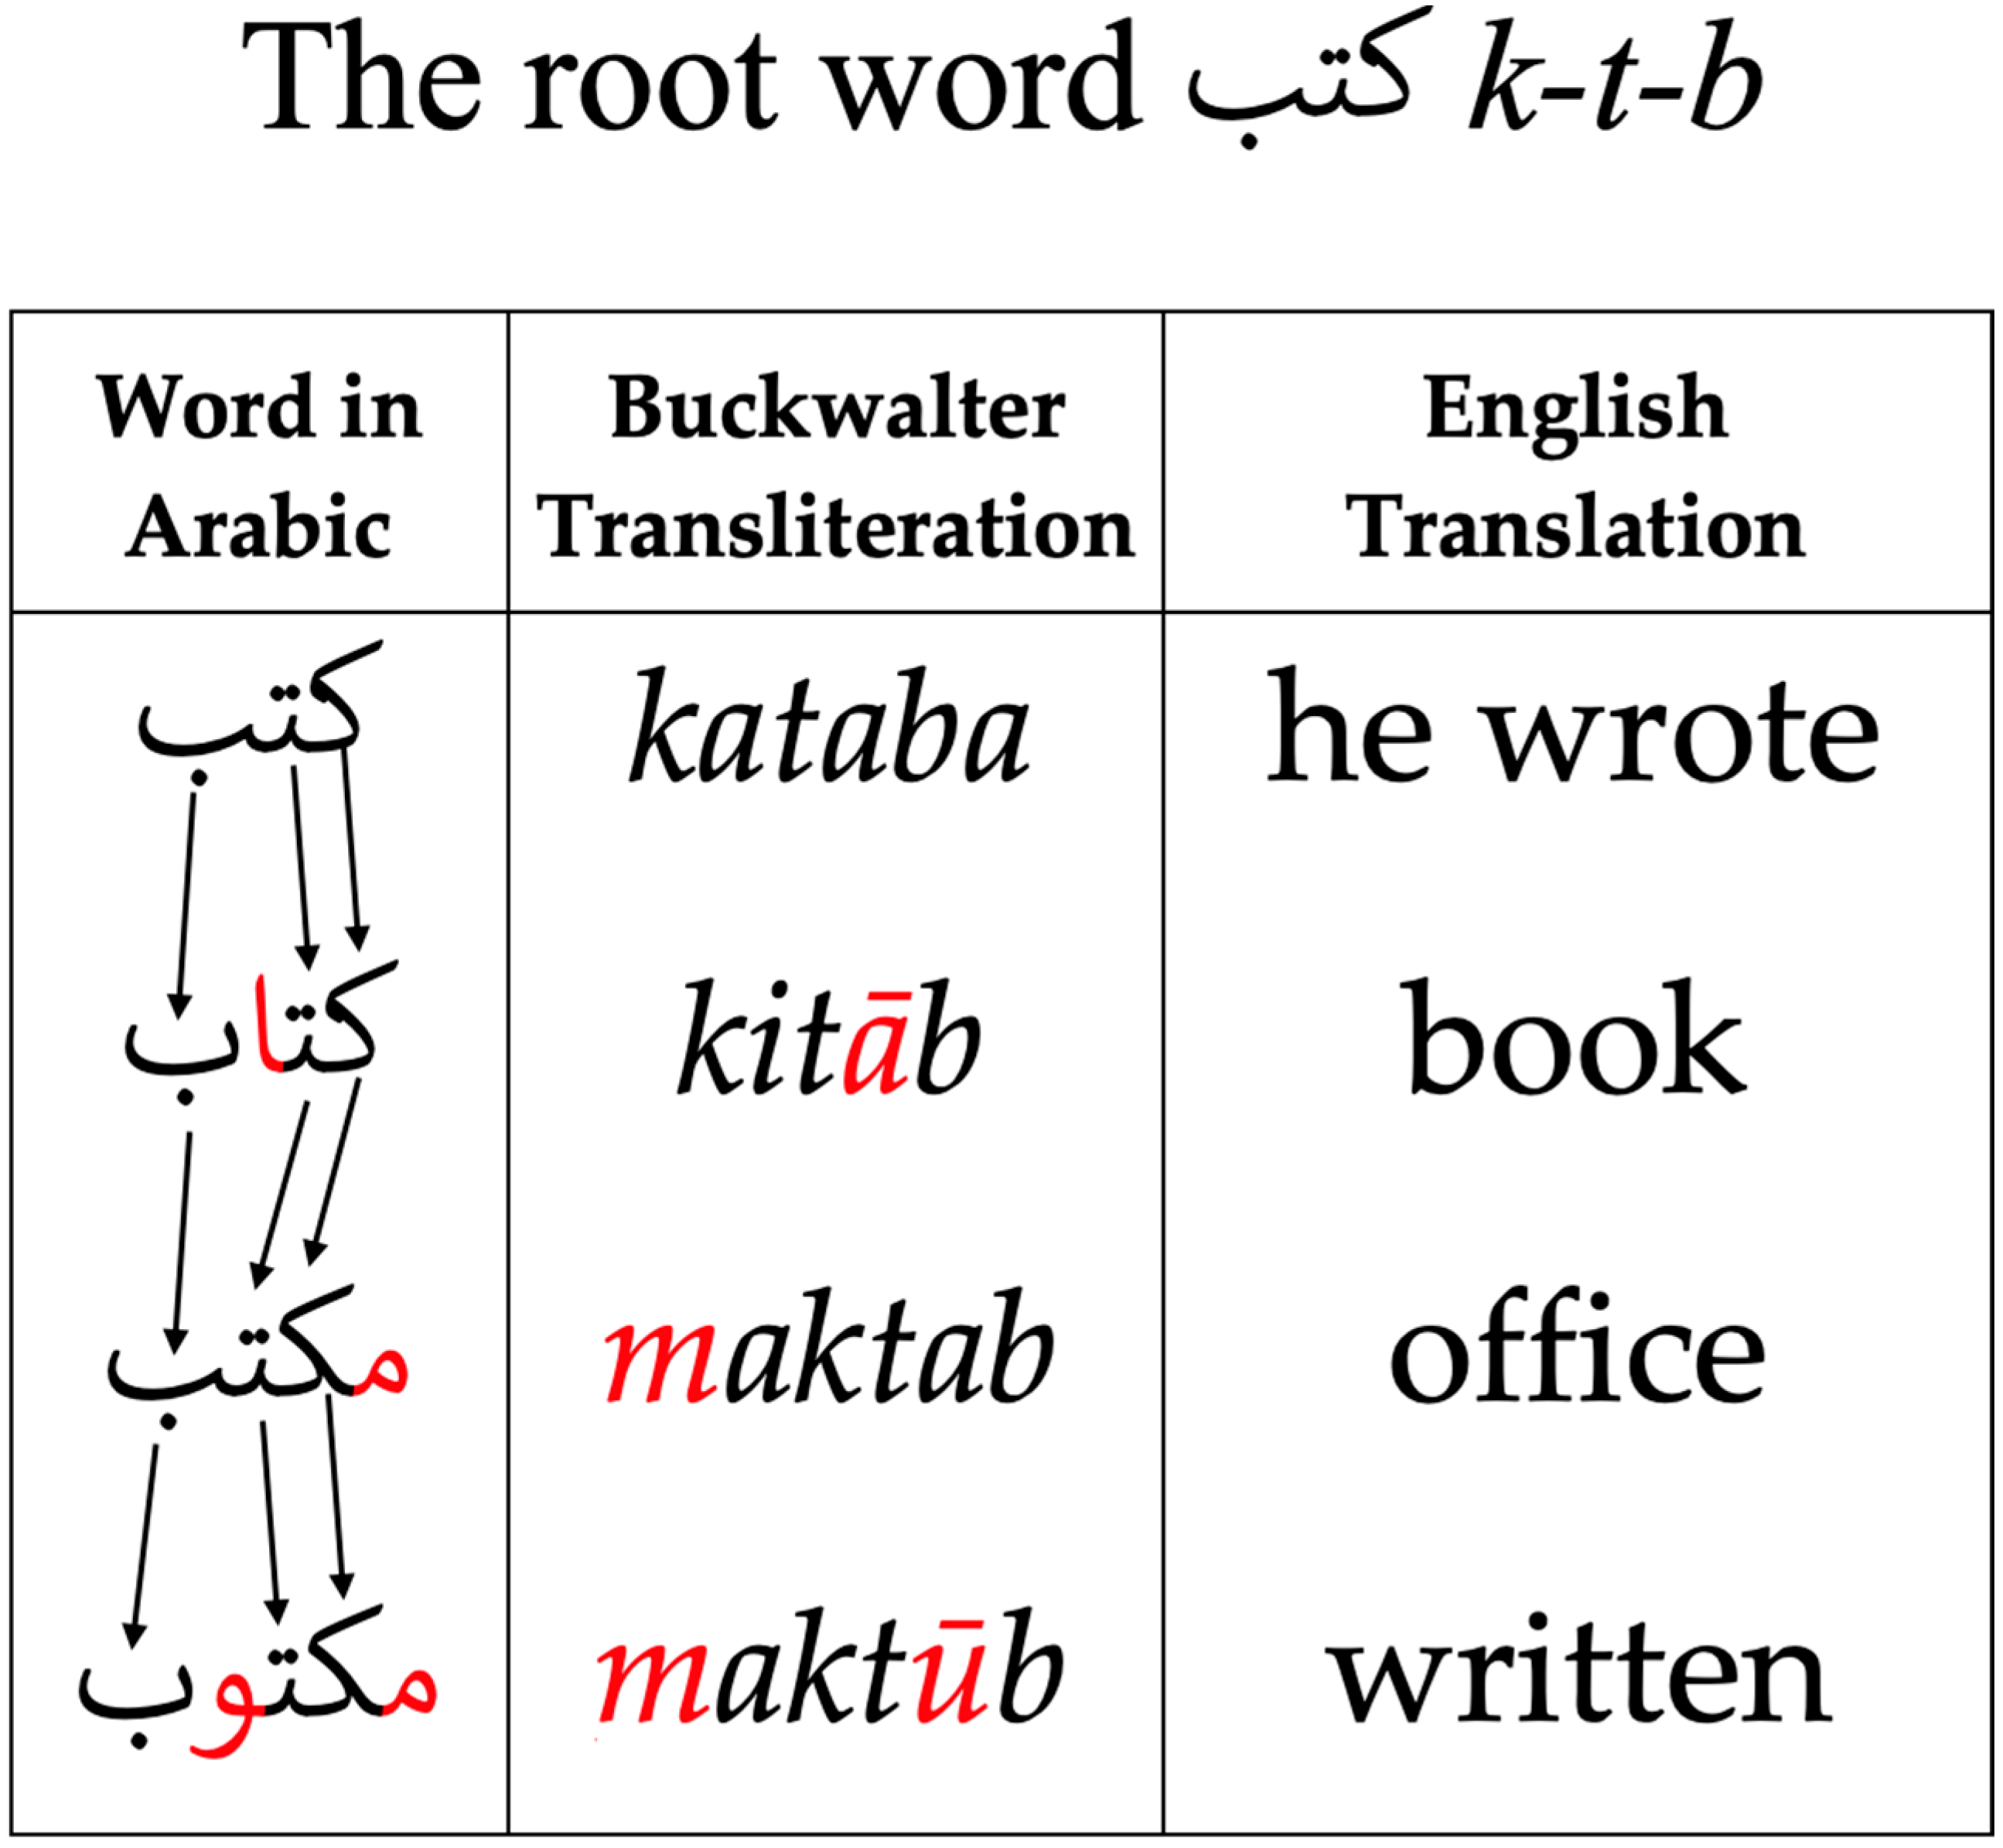
\includegraphics[width=0.72\textwidth]{morphology.png}

\caption{Example of Arabic morphological derivation from the root ``k-t-b'', illustrating the richness and complexity of Arabic word formation.}

\label{fig:arabic_morphology}

\end{figure}

\vspace{0.3cm}

In addition to root-based derivation, Arabic exhibits extensive \emph{cliticization}: function words such as the definite article, conjunctions, prepositions and pronouns are written attached to a host word. For example, the single written token \textit{walfi\d{d}\d{d}a} (``and the silver'') joins three morphological units: the conjunction \textit{wa+} (``and''), the definite article \textit{al+} (``the''), and the noun \textit{fi\d{d}\d{d}a} (``silver''). The BAREC annotation guidelines explicitly name the presence and type of clitics as markers of readability level~\cite{habash2025guidelines}, which is why making them explicit through morphological segmentation (D3Tok) is central to the methodology of this thesis.

Lexical ambiguity is another important challenge, since a single undiacritized Arabic word can correspond to several distinct readings. For example, the word \textit{`ilm}/\textit{`alam}/\textit{`allama} can mean \emph{knowledge}, \emph{flag} or \emph{he taught} depending on the context. Ambiguity has a direct effect on readability, because resolving the rarer readings requires more advanced linguistic knowledge, and the BAREC guidelines therefore place constructions that need diacritization for disambiguation at the higher readability levels. Arabic syntax also allows flexible word order, which makes sentences harder for machine learning models to understand.

Compared with English readability research, Arabic readability assessment also has few large scale annotated datasets and benchmark resources. The BAREC dataset improved this situation considerably, but fine grained readability prediction across 19 ordered levels is still a difficult task.

These challenges lead to two complementary design decisions. First, we use pretrained transformer models, whose contextual representations learned from large Arabic corpora help with the morphological, lexical and syntactic complexity. Second, we use ordinal aware learning methods to model the ordered structure of the readability levels, which standard classification ignores.
\section{Problem Statement}
Traditional readability assessment systems often treat readability prediction as a standard classification problem trained with Cross Entropy loss. Readability levels, however, are ordered by nature, and nearby levels are more similar than distant ones.

In standard classification, when the true level is 11, predicting level 10 gets exactly the same penalty as predicting level 1, although the first is a near miss and the second a far miss. Because of this, classification models cannot properly capture the ordinal structure of readability labels.

This thesis therefore investigates the following question: given a fixed AraBERTv2 backbone with D3Tok morphological segmentation and the training protocol of the BAREC benchmark, \emph{which ordinal head and loss function achieves the highest Quadratic Weighted Kappa (QWK) among cross entropy, regression with mean squared error, ordinal log loss, an Earth Mover's Distance loss, four soft label settings, a CORAL ordinal head, two regression losses with a pairwise ranking term (RANK and PLR), a conditional ordinal head (CORN) and a Soft QWK schedule in two phases; how do the loss families differ in the trade off between exact match accuracy and distance aware agreement; and are their errors near misses or far misses?}

\subsection{Research Objectives}
The main objectives of this thesis are:
\begin{itemize}

\item Determine which ordinal head and loss function give the highest QWK on the BAREC benchmark when the corpus, the encoder and the entire training protocol stay fixed.
\item Compare twelve head and loss configurations on a single AraBERTv2 and D3Tok backbone, and report the two-phase Soft-QWK schedule beside them as a separate group.

\item Test whether two regression losses with a pairwise ranking term (RANK and PLR), taken from readability research on other languages, and a conditional ordinal head (CORN) carry over to 19-level Arabic readability under the same protocol.

\item Quantify the trade off between exact-match accuracy (\textit{Acc19}) and distance aware agreement (QWK) across the loss families.

\item Measure the error distance of each method, separating near misses from far misses, as the research topic requires.

\item Establish whether a CORAL head can learn its cut points under this protocol at all, and what its cut points should be initialised to if it cannot.

\item Measure how much of the difference between published systems is due to the checkpoint selection rule and the decision threshold rather than to the loss.

\item Evaluate predictions at multiple granularities ($19$, $7$, $5$ and $3$ levels) using the BAREC collapsing scheme.

\item Compare the results with the original BAREC benchmark, with the systems of the BAREC 2025 Shared Task and with the agreement between human annotators.

\end{itemize}



\subsection{Research Contributions}
The main contributions of this thesis are:

\begin{itemize}

\item A controlled comparison of twelve head and loss configurations on one fixed pipeline, which extends the four losses of the BAREC benchmark with a CORAL ordinal head, a CORN ordinal head, two regression losses with a pairwise ranking term, four soft-label settings and a metric-aligned two-phase objective, and reports them on both official splits.
% Compare the results with the original BAREC benchmark, with the systems of the BAREC 2025 Shared Task and with the agreement between human annotators.

\item An adaptation of three objectives from outside the BAREC benchmark to 19-level Arabic readability: two regression losses with a pairwise ranking term, RANK and PLR, taken from readability research on other languages \cite{trokhymovych2024open,lee2022neural}, and the conditional ordinal head CORN \cite{shi2023deep}. None of them had been evaluated in the BAREC benchmark or by the ZAI and STBW systems, and all three run under the same protocol as the other configurations.

\item A verified reproduction of the benchmark's loss comparison, where the one visible discrepancy is explained and traced back to the checkpoint selection rule.

\item An initialisation of the CORAL cut points from the cumulative training label frequencies, motivated by how far the benchmark learning rate lets them travel. We pair it with a direct measurement of how much the cut points actually move and with two ablations that test the argument from opposite directions.
\item Two metrics of error distance, the share of predictions at least three and at least five levels away from the gold level. They separate near misses from far misses and show that the lead in QWK comes from removing far misses and not from lowering the average error.

\item A measurement of how much the checkpoint selection rule and the CORAL decision threshold are worth, which is what makes systems published under different protocols comparable.

\item A track with a frozen backbone that satisfies the CPU friendly requirement of the research topic, reports variance over five seeds and shows that the ranking of the losses on frozen features does not carry over to fine tuning.

\item A comparison of the results with the published BAREC benchmark, the systems of the BAREC 2025 Shared Task and the reported agreement between human annotators.

\end{itemize}

\subsection{Methodology Overview}
The proposed system for Arabic readability assessment combines a pretrained transformer language model with ordinal aware learning methods. The overall pipeline is shown in Figure~\ref{fig:pipeline} and proceeds as follows.

The pipeline begins with the BAREC corpus, where each Arabic sentence carries an ordered readability level from 1 to 19. The input is the D3Tok column of the corpus, a morphologically segmented form in which clitics are separated from their host word and marked with a \texttt{+}. That representation is used because AraBERTv2 was pretrained on morphologically segmented Arabic, so segmented input matches its pretraining distribution, and because the pairing of AraBERTv2 with D3Tok input is the configuration the original benchmark carries into its loss comparison \cite{elmadani2025barec}. The segmented text is tokenised and passed to AraBERTv2, and after dropout the pooled output of the encoder, a vector of 768 dimensions, is used as the sentence representation.

This representation goes to a prediction head whose form depends on the configuration. The softmax losses (cross entropy, ordinal log loss, EMD and the four soft label settings) use a linear layer with 19 outputs; regression, the Soft QWK schedule, RANK and PLR use a linear layer with a single output; CORAL uses a layer with 18 thresholds and one shared projection; and CORN uses a layer with 18 outputs, one for each conditional threshold. During training, the corresponding loss compares the output of the head with the gold label. At inference, the output is decoded to a level between 1 and 19 by taking the highest score, by rounding, or by counting how many thresholds are exceeded. Every configuration is trained and evaluated under the same protocol, with QWK as the primary metric, together with exact accuracy (\textit{Acc19}), adjacent accuracy ($\pm 1$ \textit{Acc19}), average distance (\textit{Dist}), the collapsed $7$-, $5$- and $3$-level accuracies, and the two error-distance metrics introduced in this thesis.
\begin{figure}[tbp]
    \centering
    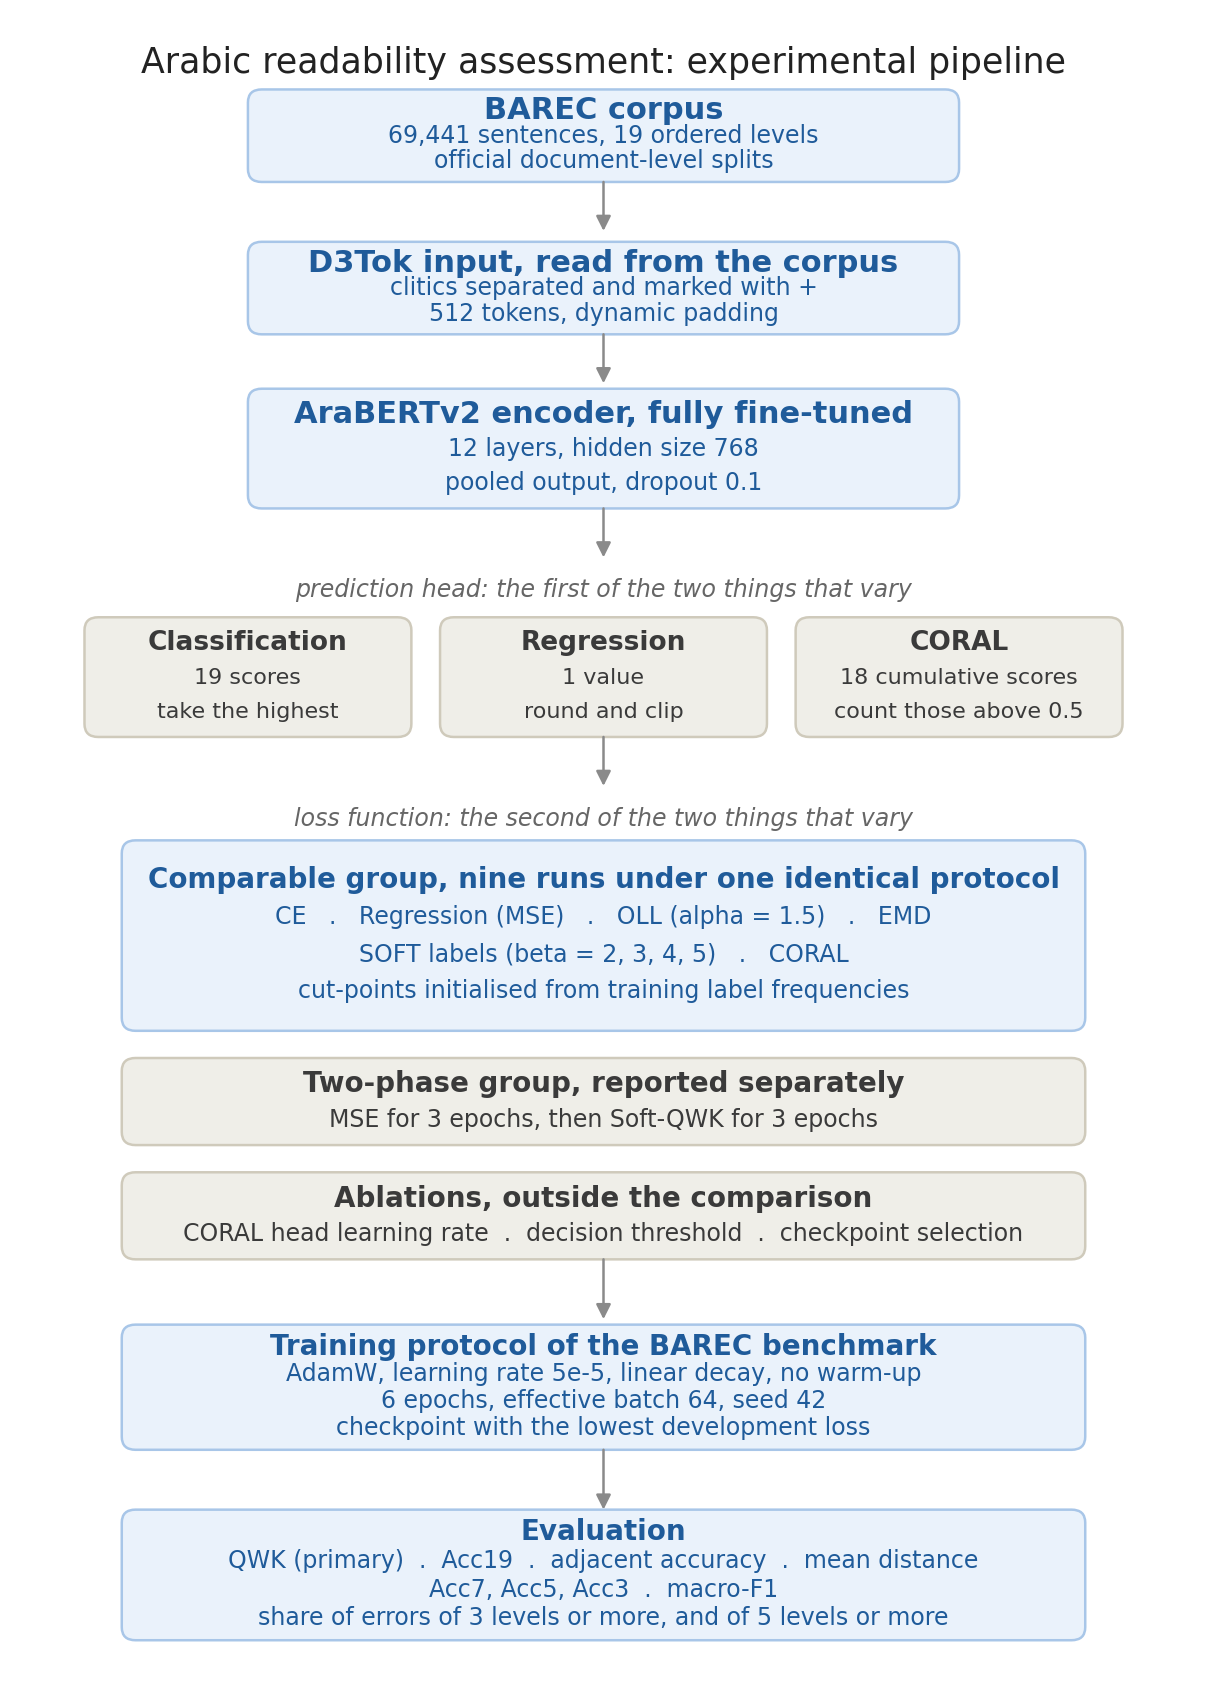
\includegraphics[width=0.78\linewidth]{pipeline.png}
    \caption{The experimental pipeline. Everything drawn in blue is held fixed for every run; the prediction head and the loss function, drawn in grey, are the only components that vary.}
    \label{fig:pipeline}
\end{figure}
\vspace{0.3cm}


\subsection{Thesis Organization}

This thesis is organized as follows:

\vspace{0.3cm}

\begin{itemize}

\item \textbf{Chapter 1 -- Introduction:}
This chapter introduces the background and motivation of Arabic readability assessment. It also presents the research objectives, the challenges, the contributions, an overview of the methodology and the evaluation metrics used in this work.

\vspace{0.2cm}

\item \textbf{Chapter 2 -- Literature Review:}
This chapter reviews previous studies related to Arabic readability assessment, Arabic NLP challenges, pretrained language models, ordinal regression methods, pairwise ranking objectives for readability, and systems developed using the BAREC dataset.

\vspace{0.2cm}

\item \textbf{Chapter 3 -- Proposed Methodology:}
This chapter describes the corpus and its splits, the D3Tok input representation, the encoder and the prediction heads, and the exact form of every loss function with the tests that verify it. It then covers the initialisation of the CORAL cut points, the training protocol with every declared difference from the published script, the evaluation metrics and the track with a frozen backbone.
\vspace{0.2cm}

\item \textbf{Chapter 4 -- Experiments and Results:}
This chapter reports the integrity checks, the reproduction of the published benchmark and the full results of the fourteen runs on both splits, including RANK, PLR and CORN. It then examines the trade off between exact accuracy and ordinal agreement, the analysis of error distance, the three ablations of the fine-tuning track, the track with a frozen backbone and its own ablation, and ends with a comparison against published systems and human agreement, followed by the limitations.

\vspace{0.2cm}

\item \textbf{Chapter 5 -- Conclusion and Future Work:}
The final chapter brings the findings together, states the contributions and the limitations, and sets out the next steps. The first of these is a study over multiple seeds, which would turn the leading group from an observation into a measurement.
\end{itemize}

\section{Summary of Introduction}
This chapter introduced the context of Arabic readability assessment and the challenges that make it harder than English readability, namely morphological richness, lexical ambiguity and syntactic complexity. It then stated the research question, which asks which ordinal head and loss function gives the highest QWK on BAREC when the protocol is held fixed, and whether the errors are near misses or far misses. It also listed the twelve configurations compared, the nine of the comparable group and the three added objectives RANK, PLR and CORN, together with the Soft QWK schedule in two phases reported next to them and the ablations. The methodology overview described the AraBERTv2 and D3Tok pipeline and the evaluation metrics.
\textit{The next chapter reviews previous work on readability assessment, pretrained language models, the BAREC corpus, ordinal regression methods, pairwise ranking objectives for readability and the systems built for the BAREC 2025 Shared Task.}
